\chapter{Reihungstest}

Die Seite zum Starten eines Reihungstests findet sich unter /cis/testtool/index.html

\begin{figure}
	\centering
	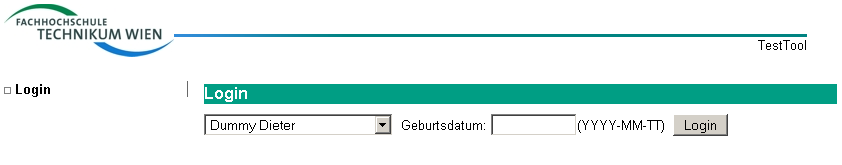
\includegraphics[width=0.75\textwidth]{testtool_login.png}
	\caption{Testtool Login}
	\label{Testtool Login}
\end{figure}

Zum Einloggen muss der Interessent ausgew�hlt werden, und das Geburtsdatum des Interessenten eingetragen werden.

\begin{figure}
	\centering
	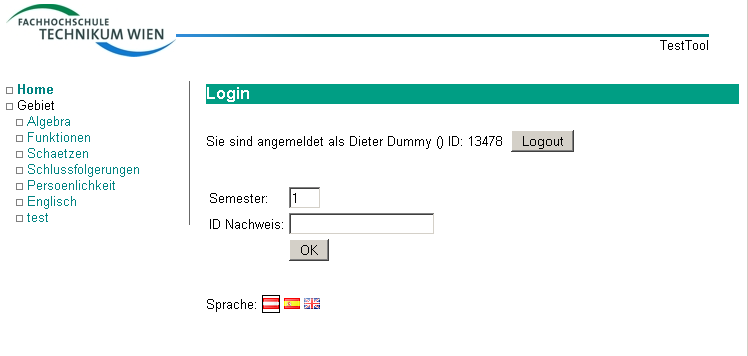
\includegraphics[width=0.75\textwidth]{testtool_login2.png}
	\caption{Testtool Einstellungen}
	\label{Testtool Einstellungen}
\end{figure}

In der folgenden Seite kann das Semester ausgew�hlt werden, f�r das der Reihungstest absolviert werden soll. Dies wird automatisch mit den Informationen aus dem FAS bef�llt und sollte in der Regel richtig bef�llt sein.\\
Im Unteren Teil, kann die Sprache ausgew�hlt werden, in der die Fragen und Vorschl�ge angezeigt werden. Diese Option steht nur dann zur Verf�gung, wenn beim Studiengang das Attribut testtool\_sprachwahl gesetzt ist. Standardm��ig ist die Sprache des Studienganges vorausgew�hlt.\\

\section{Starten eines Gebiets}

Im linken Men� scheinen nun die zugeteilten Gebiete auf.\\

\achtung{Wenn eines der Gebiete rot markiert ist, dann befinden sich Fehler in der Zusammenstellung des Gebietes. In diesem Fall starten Sie die Pr�fung in der Adminseite und beheben Sie die angezeigten Fehler.}\\
\\
\\
Beim Anklicken des Gebietes wird die Infoseite des Gebietes angezeigt (Frage mit der Nummer 0). Mit einem klick auf 'weiter' k�nnen die Demos zu diesem Gebiet angezeigt werden.\\
\\
Um das Gebiet zu starten, dr�cken Sie rechts oben auf 'Start'. Sobald das Gebiet gestartet ist, beginnt auch die Zeit zu laufen. Wenn die Zeit abgelaufen ist, wird das Gebiet automatisch beendet.

\begin{figure}
	\centering
	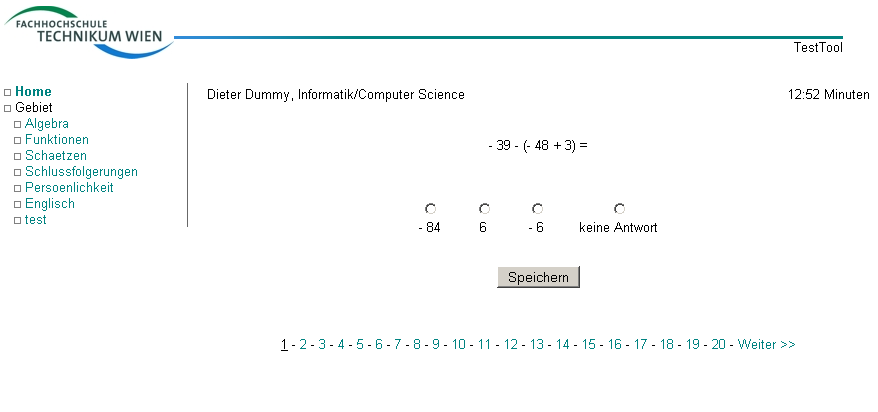
\includegraphics[width=0.75\textwidth]{testtool_frage.png}
	\caption{Beantworten von Fragen}
	\label{Beantworten von Fragen}
\end{figure}

Es werden nun nacheinander die Fragen angezeigt. Um die Frage zu beantworten markieren sie die Antwort und dr�cken auf Speichern. Nach dem Speichern wird automatisch die n�chste Frage angezeigt.

